\section{Results}
\subsection{RESU Results}
\label{sec:Flight-Results}

% Graphs will be presented in this order: 
%	1. Temp 1,2,6 					temperatures.jpg
%	2. Exterior Thermal Couple		hasp-thermal-couple.png		
%	3.Humidity					    humidity.png
%	4. Pressure					    pressure.png
%	5. BNO 						    theta-xyz.png
%	6. Magnetometer				    magnetometer.png
%	7. Orientation					orientation-xyz.png
%	8. Heading					    heading.png
%	9. Satellite Count				SAT_COUNT.jpg
%	10. Electrical Profile			payload-10-electrical-profile.png

The following figures include our data from RESU for the duration of the flight. Total flight time duration was \SI{10}{\hour}, \SI{38}{\minute}, and \SI{4}{\second}.

Three analog temperature sensors were placed at locations inside the payload, on the pump, and on the MiniPIX.  Figure~\ref{fig:Temperatures} depicts the ambient temperature in \textcolor{red}{red}, pump temperature in \textcolor{green}{green}, and the external MiniPIX temperature in \textcolor{blue}{blue}, with Mountain Standard timestamps. A total of \num{15203} data entries were record during flight.

\begin{figure}[H]
\centering
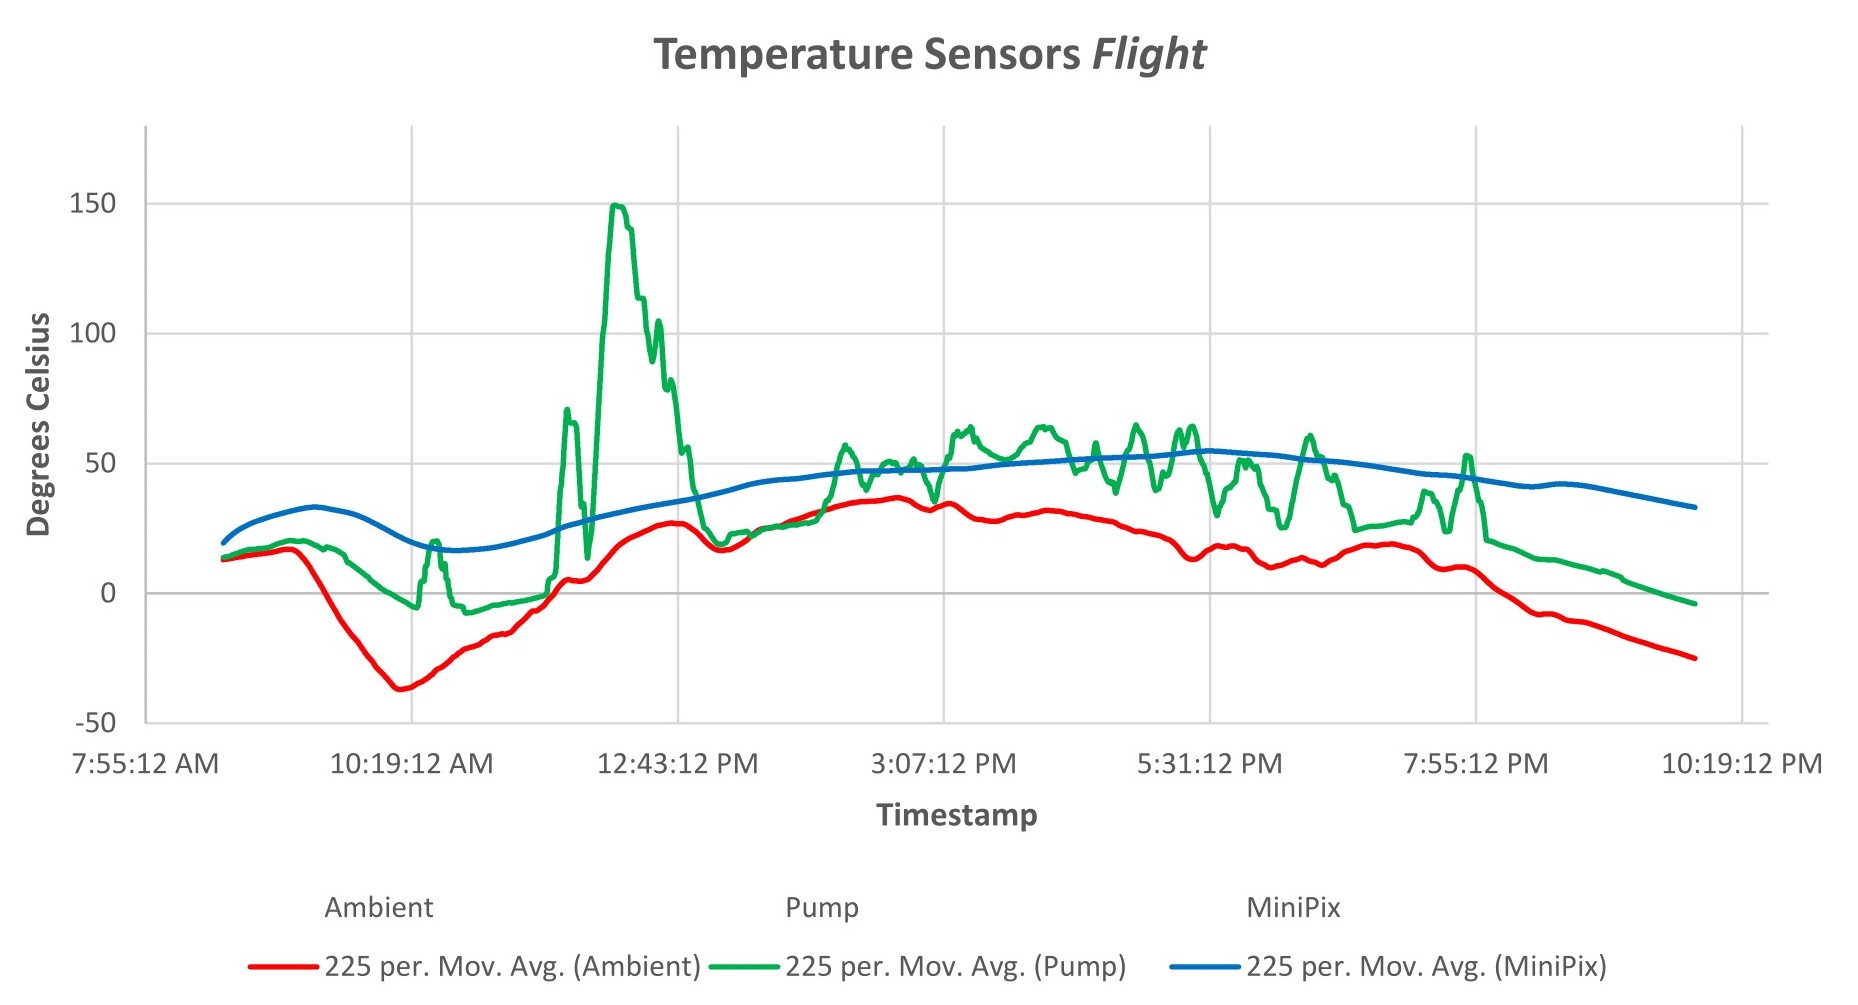
\includegraphics[width=\textwidth, keepaspectratio]{./Figures/temperatures.jpg}
\caption{Temperature readings from the interior of the payload, the pump, and MiniPIX detector.}
\label{fig:Temperatures}
\end{figure}
%-- 
\clearpage
A thermocouple was placed on the outside wall of our payload.  The HASP team provided this as another resource to monitor the temperatures of the environment.  Figure~\ref{fig:Thermal-Couple} depicts the temperatures recorded over Universal Standard timestamps in $MM$/$DD$/$YY$ $HH$:$MM$ format. 

\begin{figure}[H]
\centering
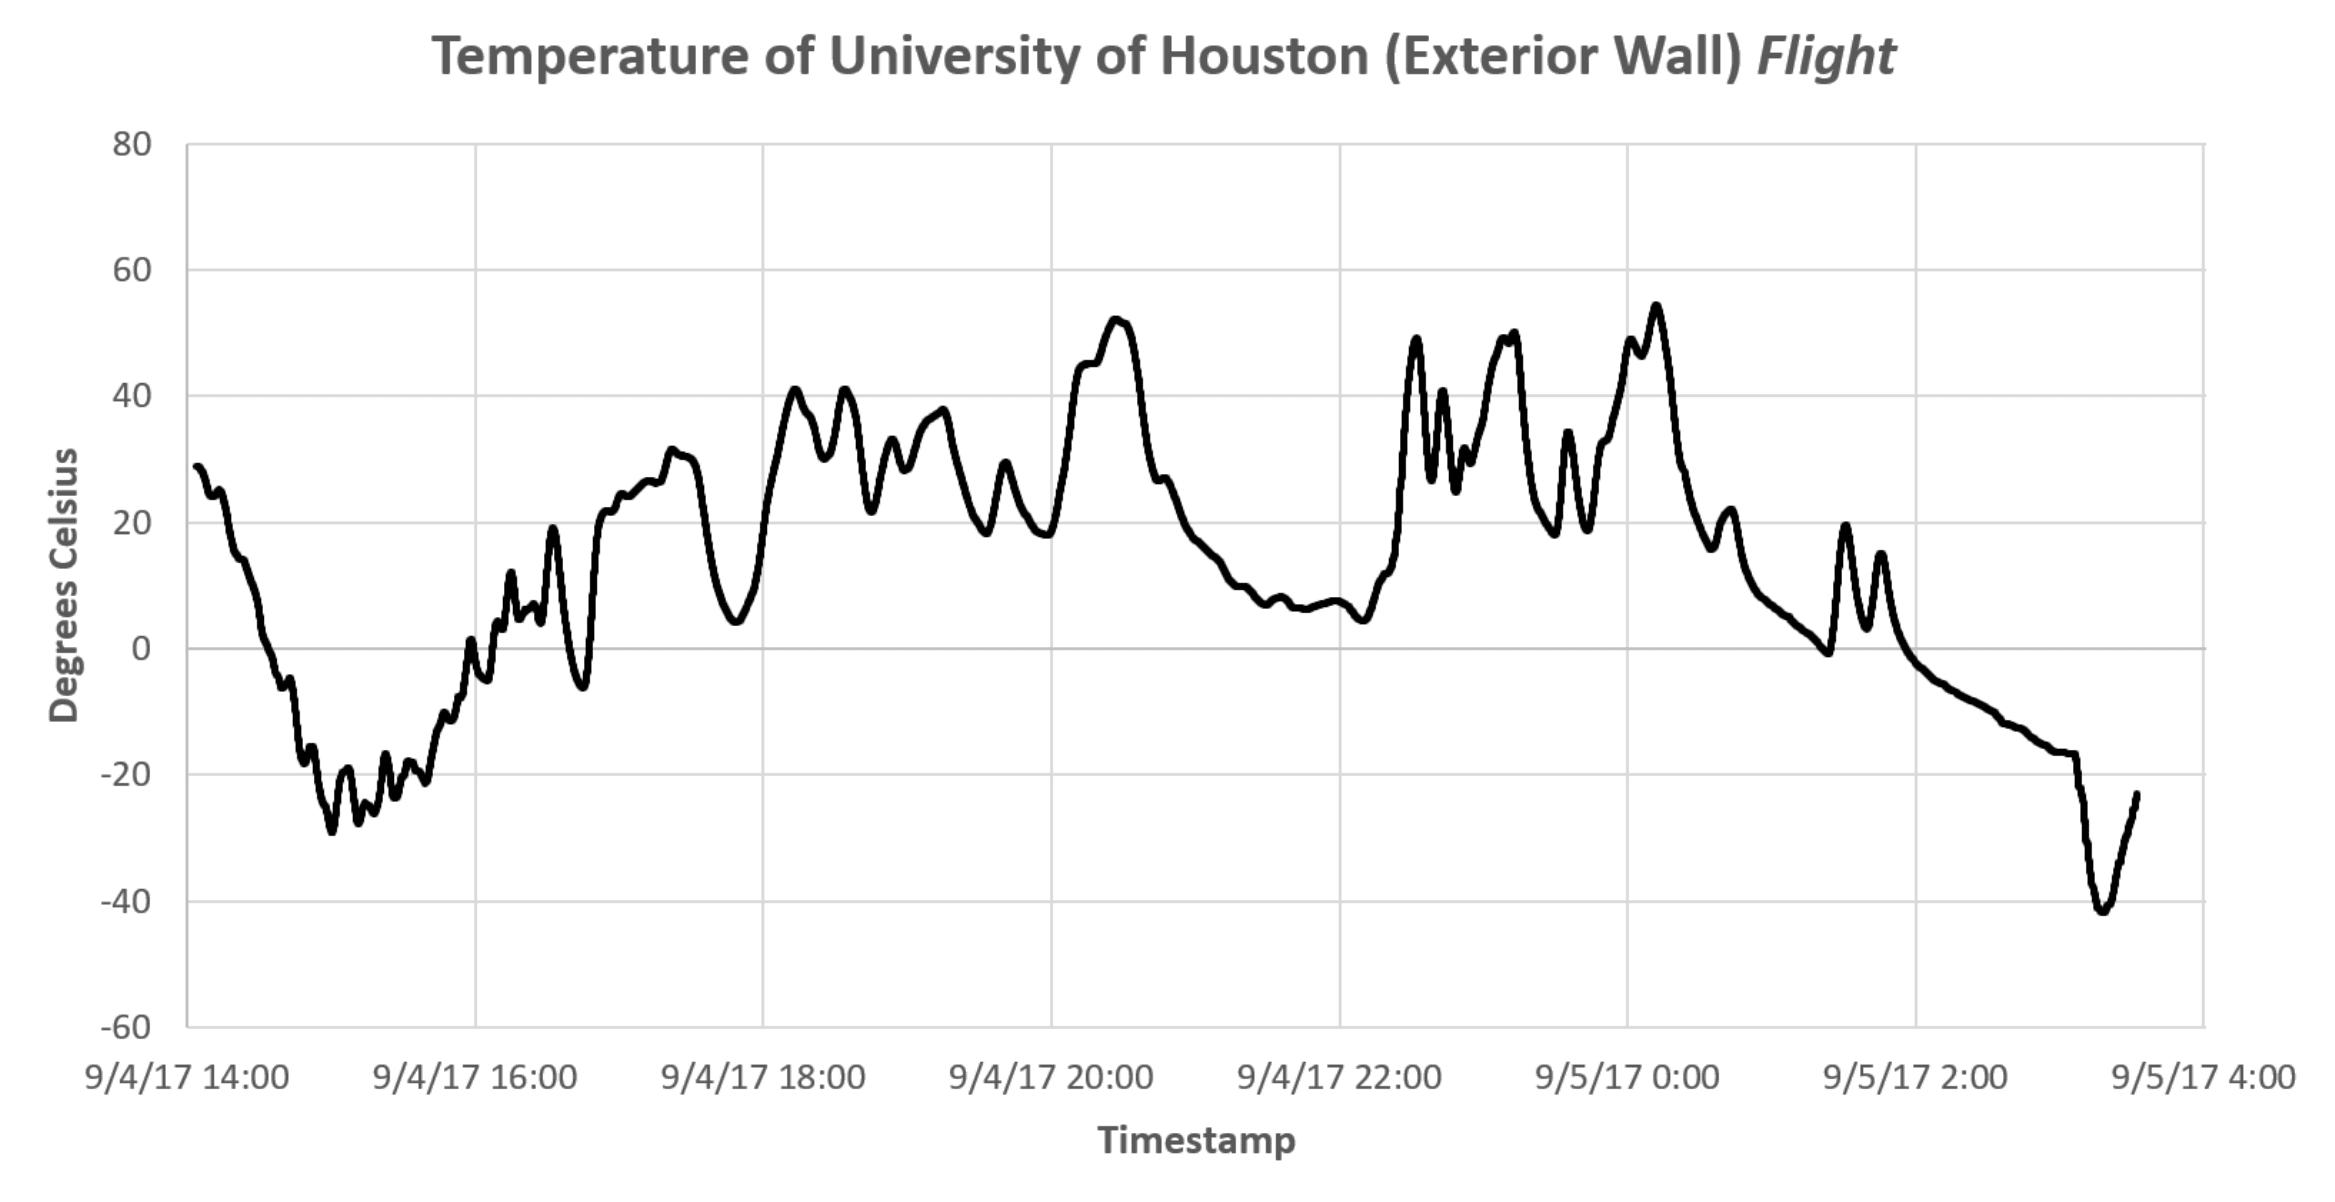
\includegraphics[width=\textwidth, keepaspectratio]{./Figures/hasp-thermal-couple.png}
\caption{Temperature from the outside wall of the SORA payload provided by the HASP thermocouple.}
\label{fig:Thermal-Couple} 
\end{figure}
%-- 

Figure~\ref{fig:Humidity} depicts a digital humidity sensor that recorded relative humidity over Mountain Standard timestamps.  A total of \num{15203} data entries were record during flight.

\begin{figure}[h]
\centering
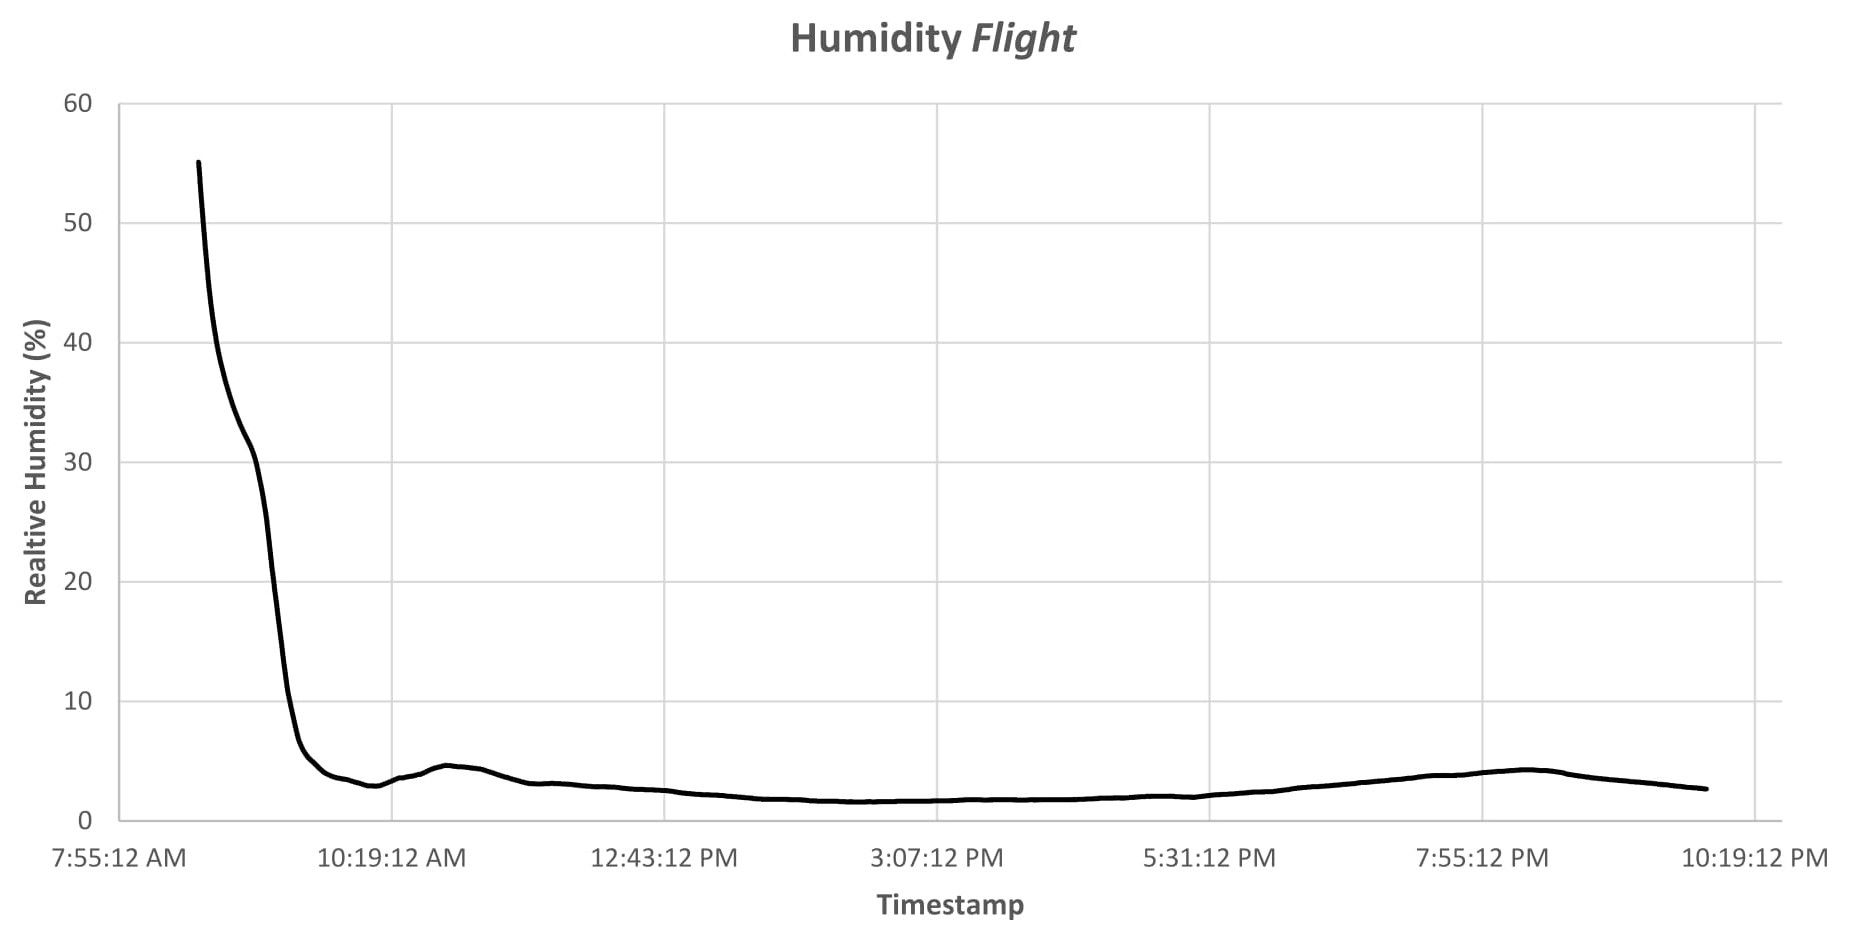
\includegraphics[width=\textwidth]{./Figures/humidity.jpg}
\caption{Digital humidity sensor data during flight.}
\label{fig:Humidity} 
\end{figure}
%-- 
\clearpage
Figure~\ref{fig:Pressure} depicts a digital pressure sensor that was also placed within the payload that too recorded pressure in millibars over Mountain Standard timestamps.  A total of \num{15203} data entries were record during flight.

\begin{figure}[h!]
\centering
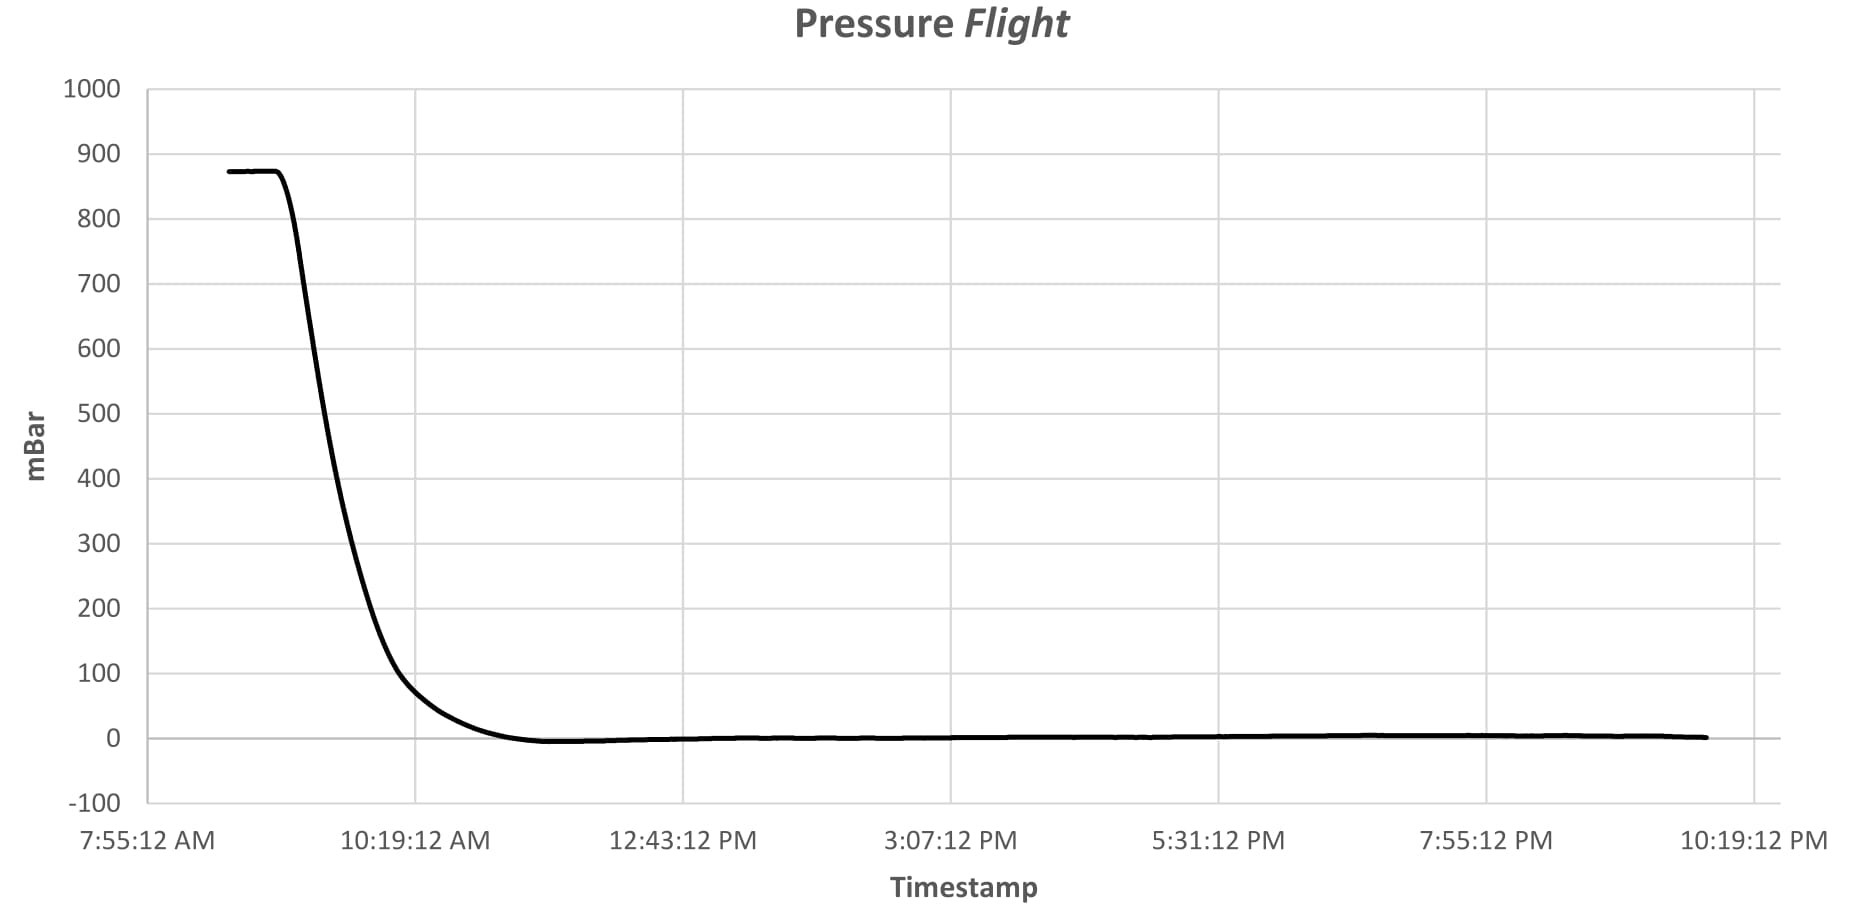
\includegraphics[width=\textwidth]{./Figures/pressure.jpg}
\caption{Digital pressure sensor data during flight.}
\label{fig:Pressure} 
\end{figure}
%-- 
Figure~\ref{fig:Electrical-Profile} depicts the current and voltage consumption during flight.  This was provided by the HASP team which we monitored live during flight. 

\begin{figure}[H]
\centering
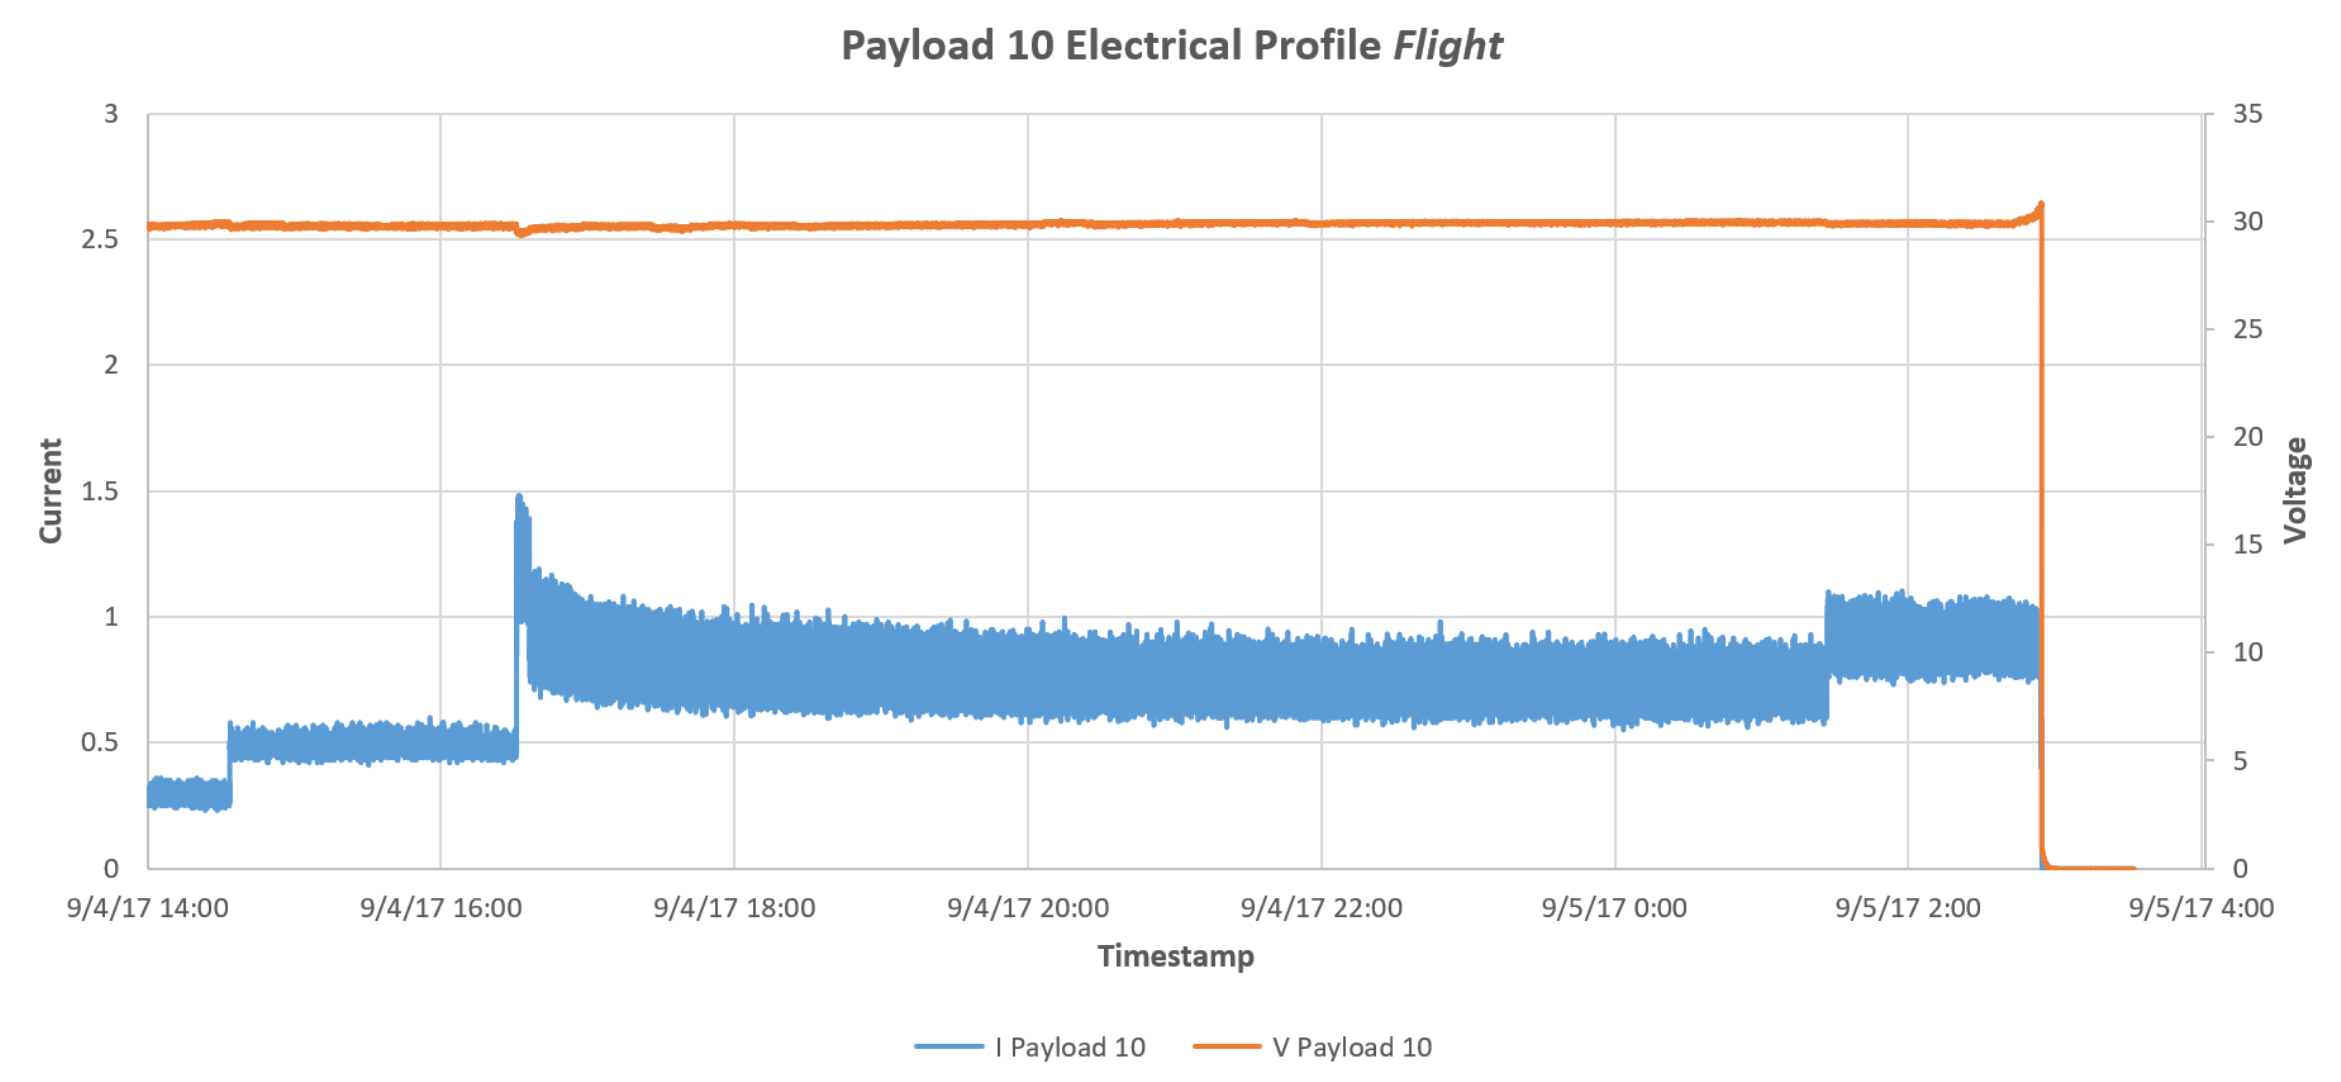
\includegraphics[height=9cm, width=\textwidth]{./Figures/payload-10-electrical-profile}
\caption{Current and voltage consumption of our payload as provided by the HASP team.}
\label{fig:Electrical-Profile}
\end{figure}
%--

\clearpage
Figure~\ref{fig:BNO} depicts the movement of the payload through three dimensions, in degrees, using the BNO 6055 and across Mountain Standard timestamps.  Data from the embedded accelerometer and gyroscope were used to create a summary of the payload's movement during flight.  A total of \num{359969} data entries were recorded during flight. 

\begin{figure}[H]
\centering
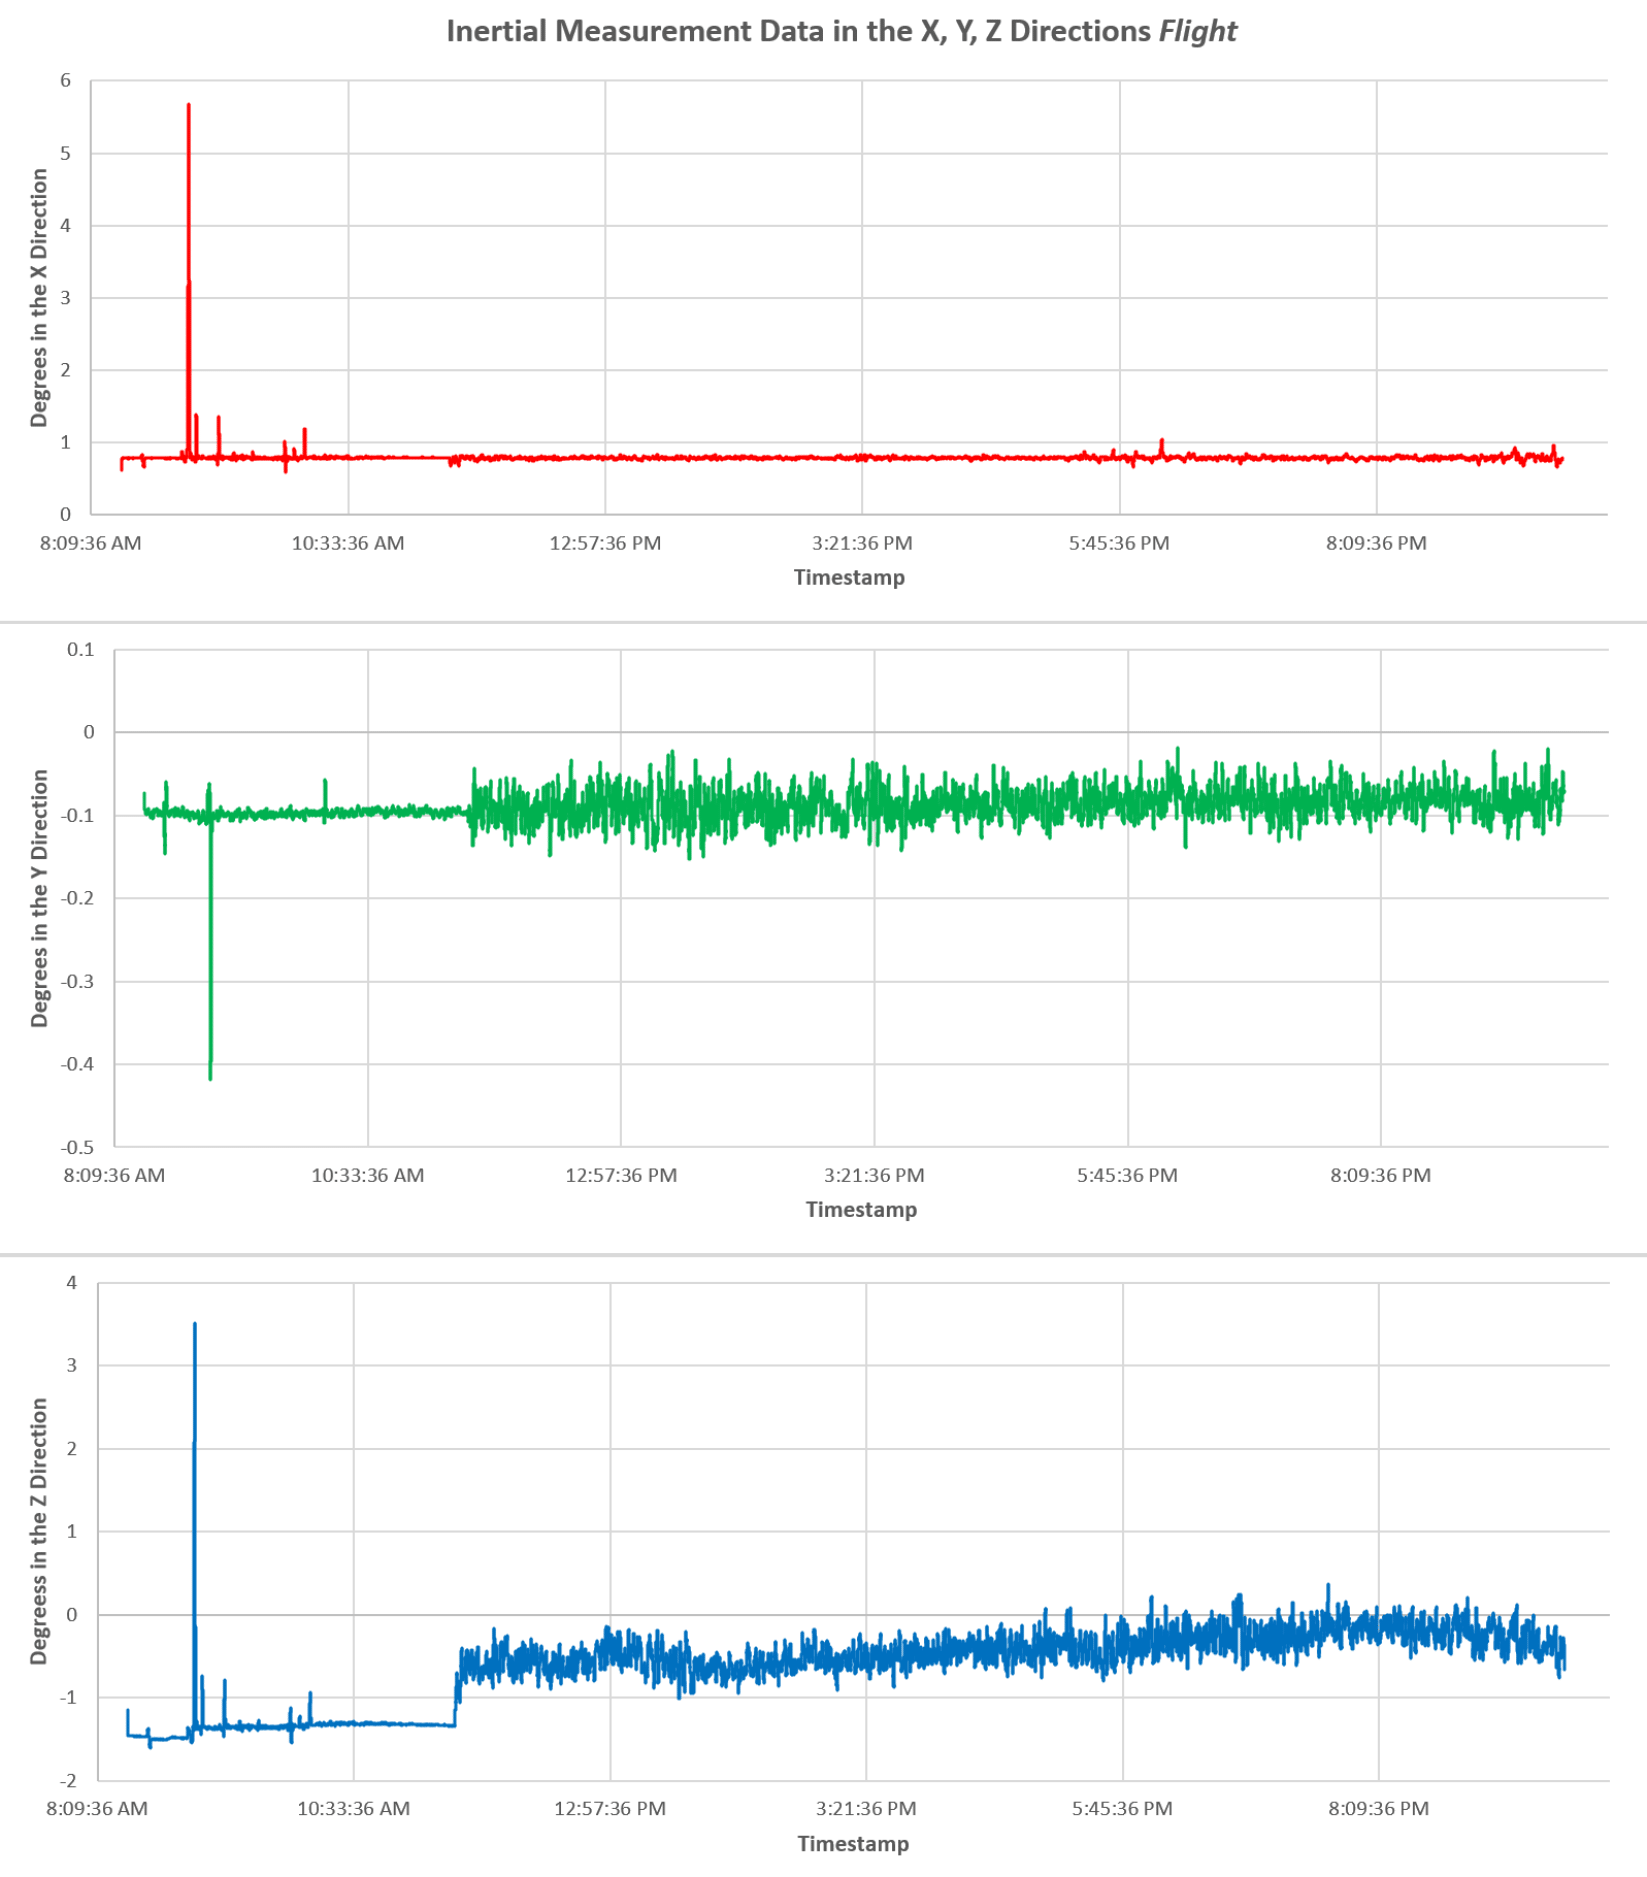
\includegraphics[width=\textwidth]{./Figures/theta-xyz.png}
\caption{Rotation of the SORA payload in the $x, y, z$ directions.}
\label{fig:BNO} 
\end{figure}
\clearpage
%-- 

Figure~\ref{fig:Magnetometer} depicts the magnetic field induced in three dimensions in micro-Teslas using the BNO 6055 over Mountain Standard timestamps.  Data from the embedded magnetometer was used to create a summary of the magnetic field experienced within the payload.  A total of \num{359969} data entries were recorded during flight. 

\begin{figure}[H]
\centering
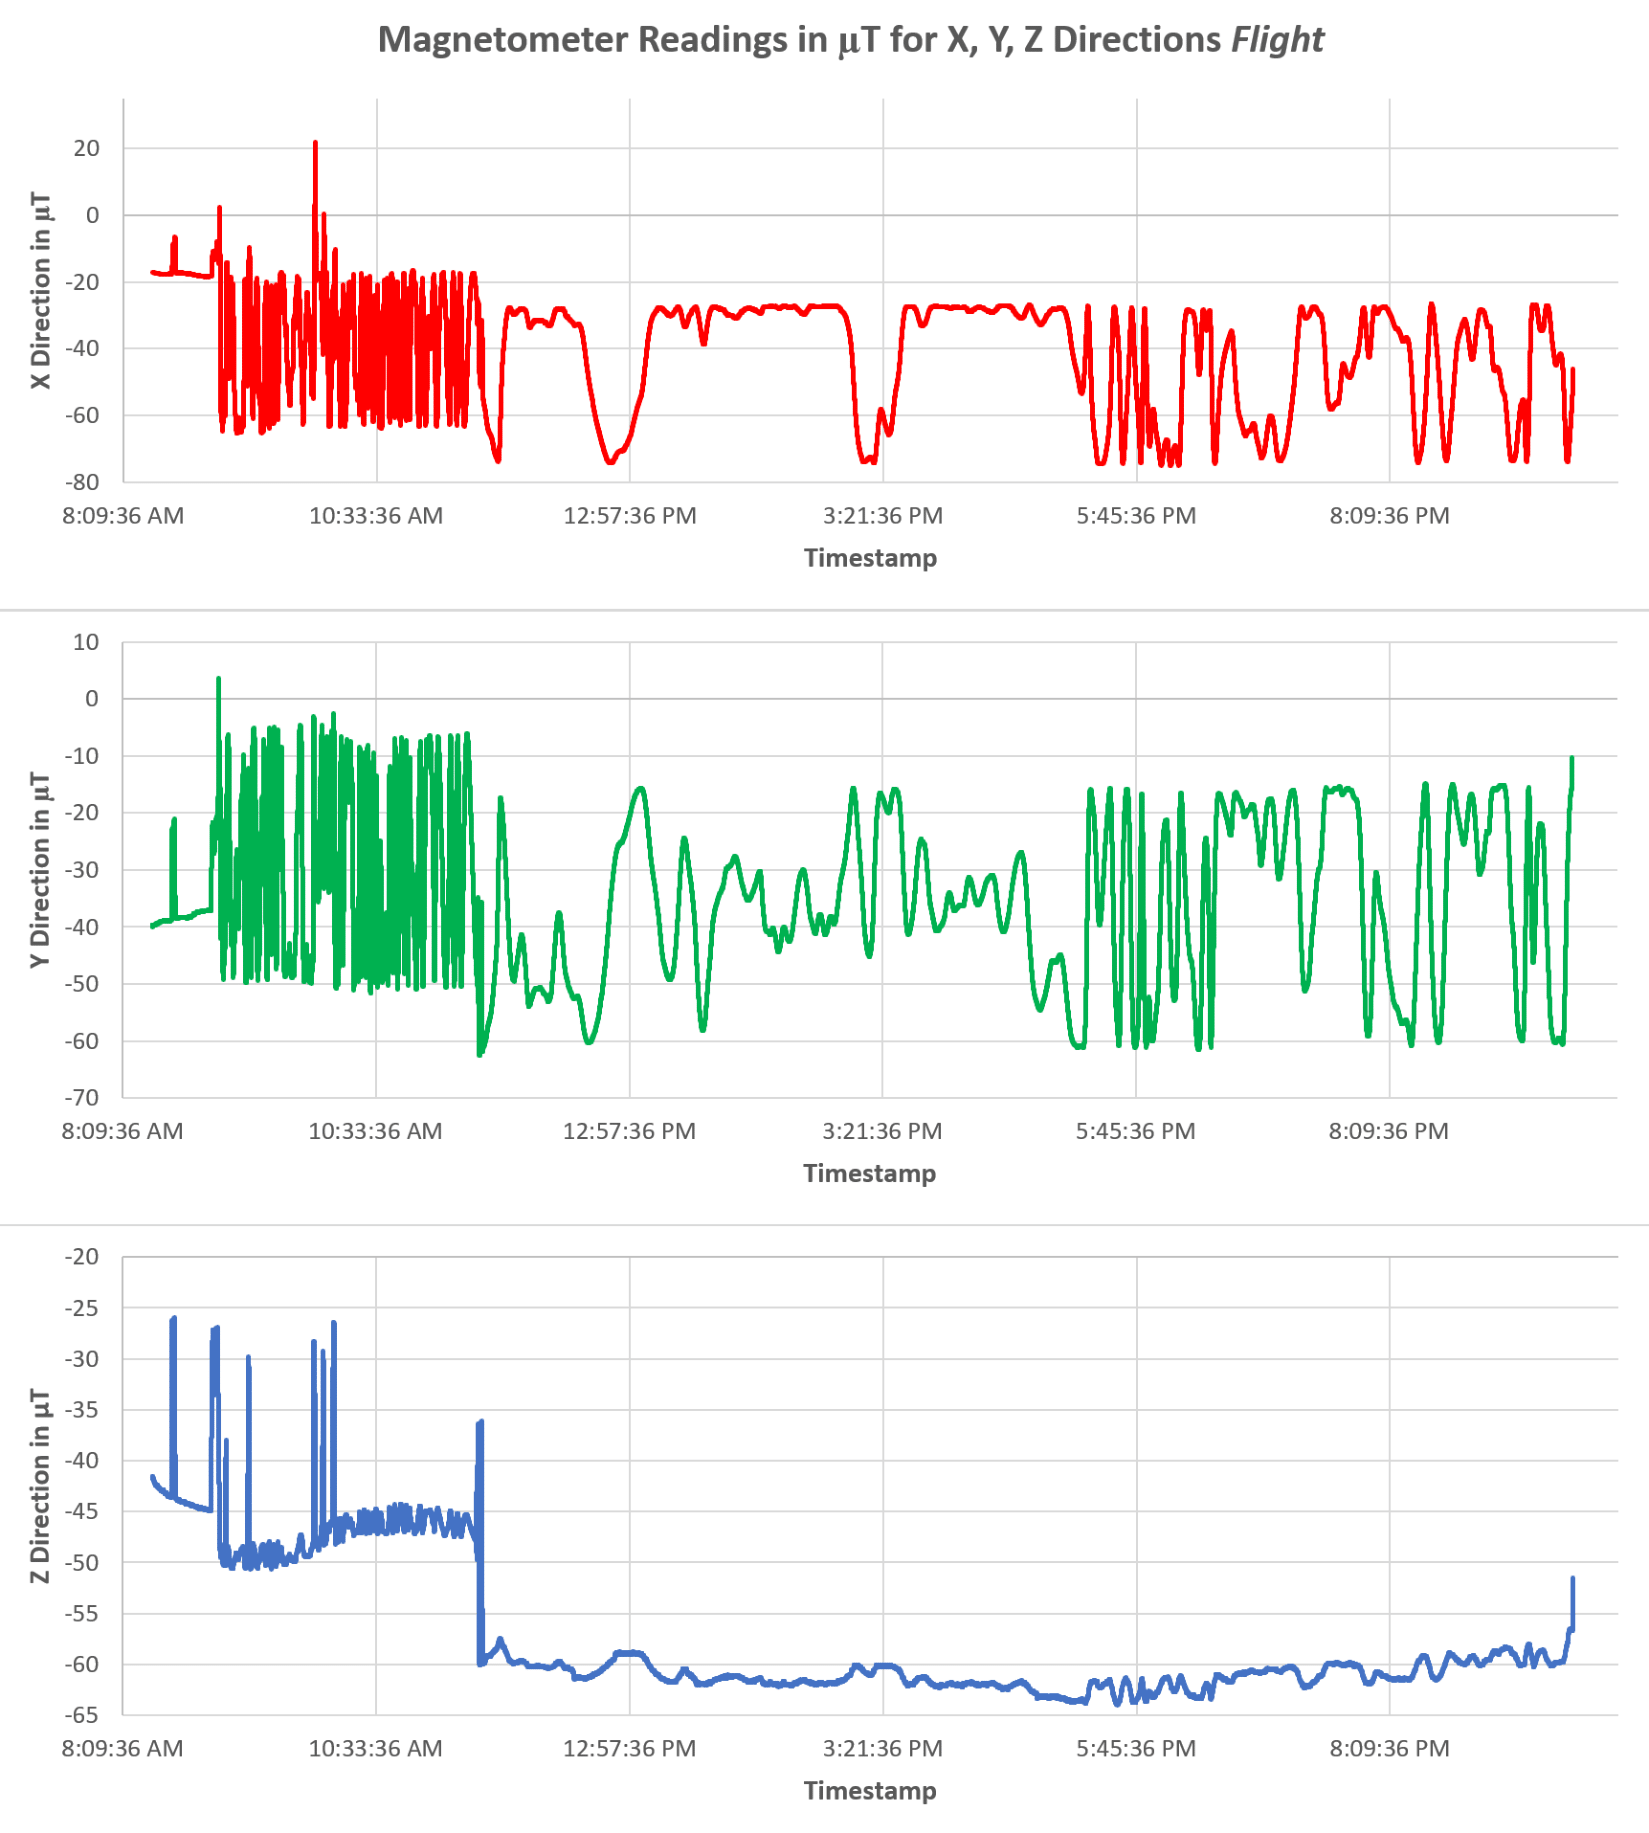
\includegraphics[width=\textwidth]{./Figures/magnetometer.png}
\caption{Magnetic field Induced within the SORA payload in the $x, y, z$ directions.}
\label{fig:Magnetometer} 
\end{figure}
\clearpage
%--

Figure~\ref{fig:Orientation} depicts the orientation of the payload through three dimensions in degrees using the BNO 6055 over Mountain Standard timestamps.  Data from the embedded magnetometer was used to summarize the payloads orientation in three space.  A total of \num{359969} data entries were recorded during flight. 

\begin{figure}[H]
\centering
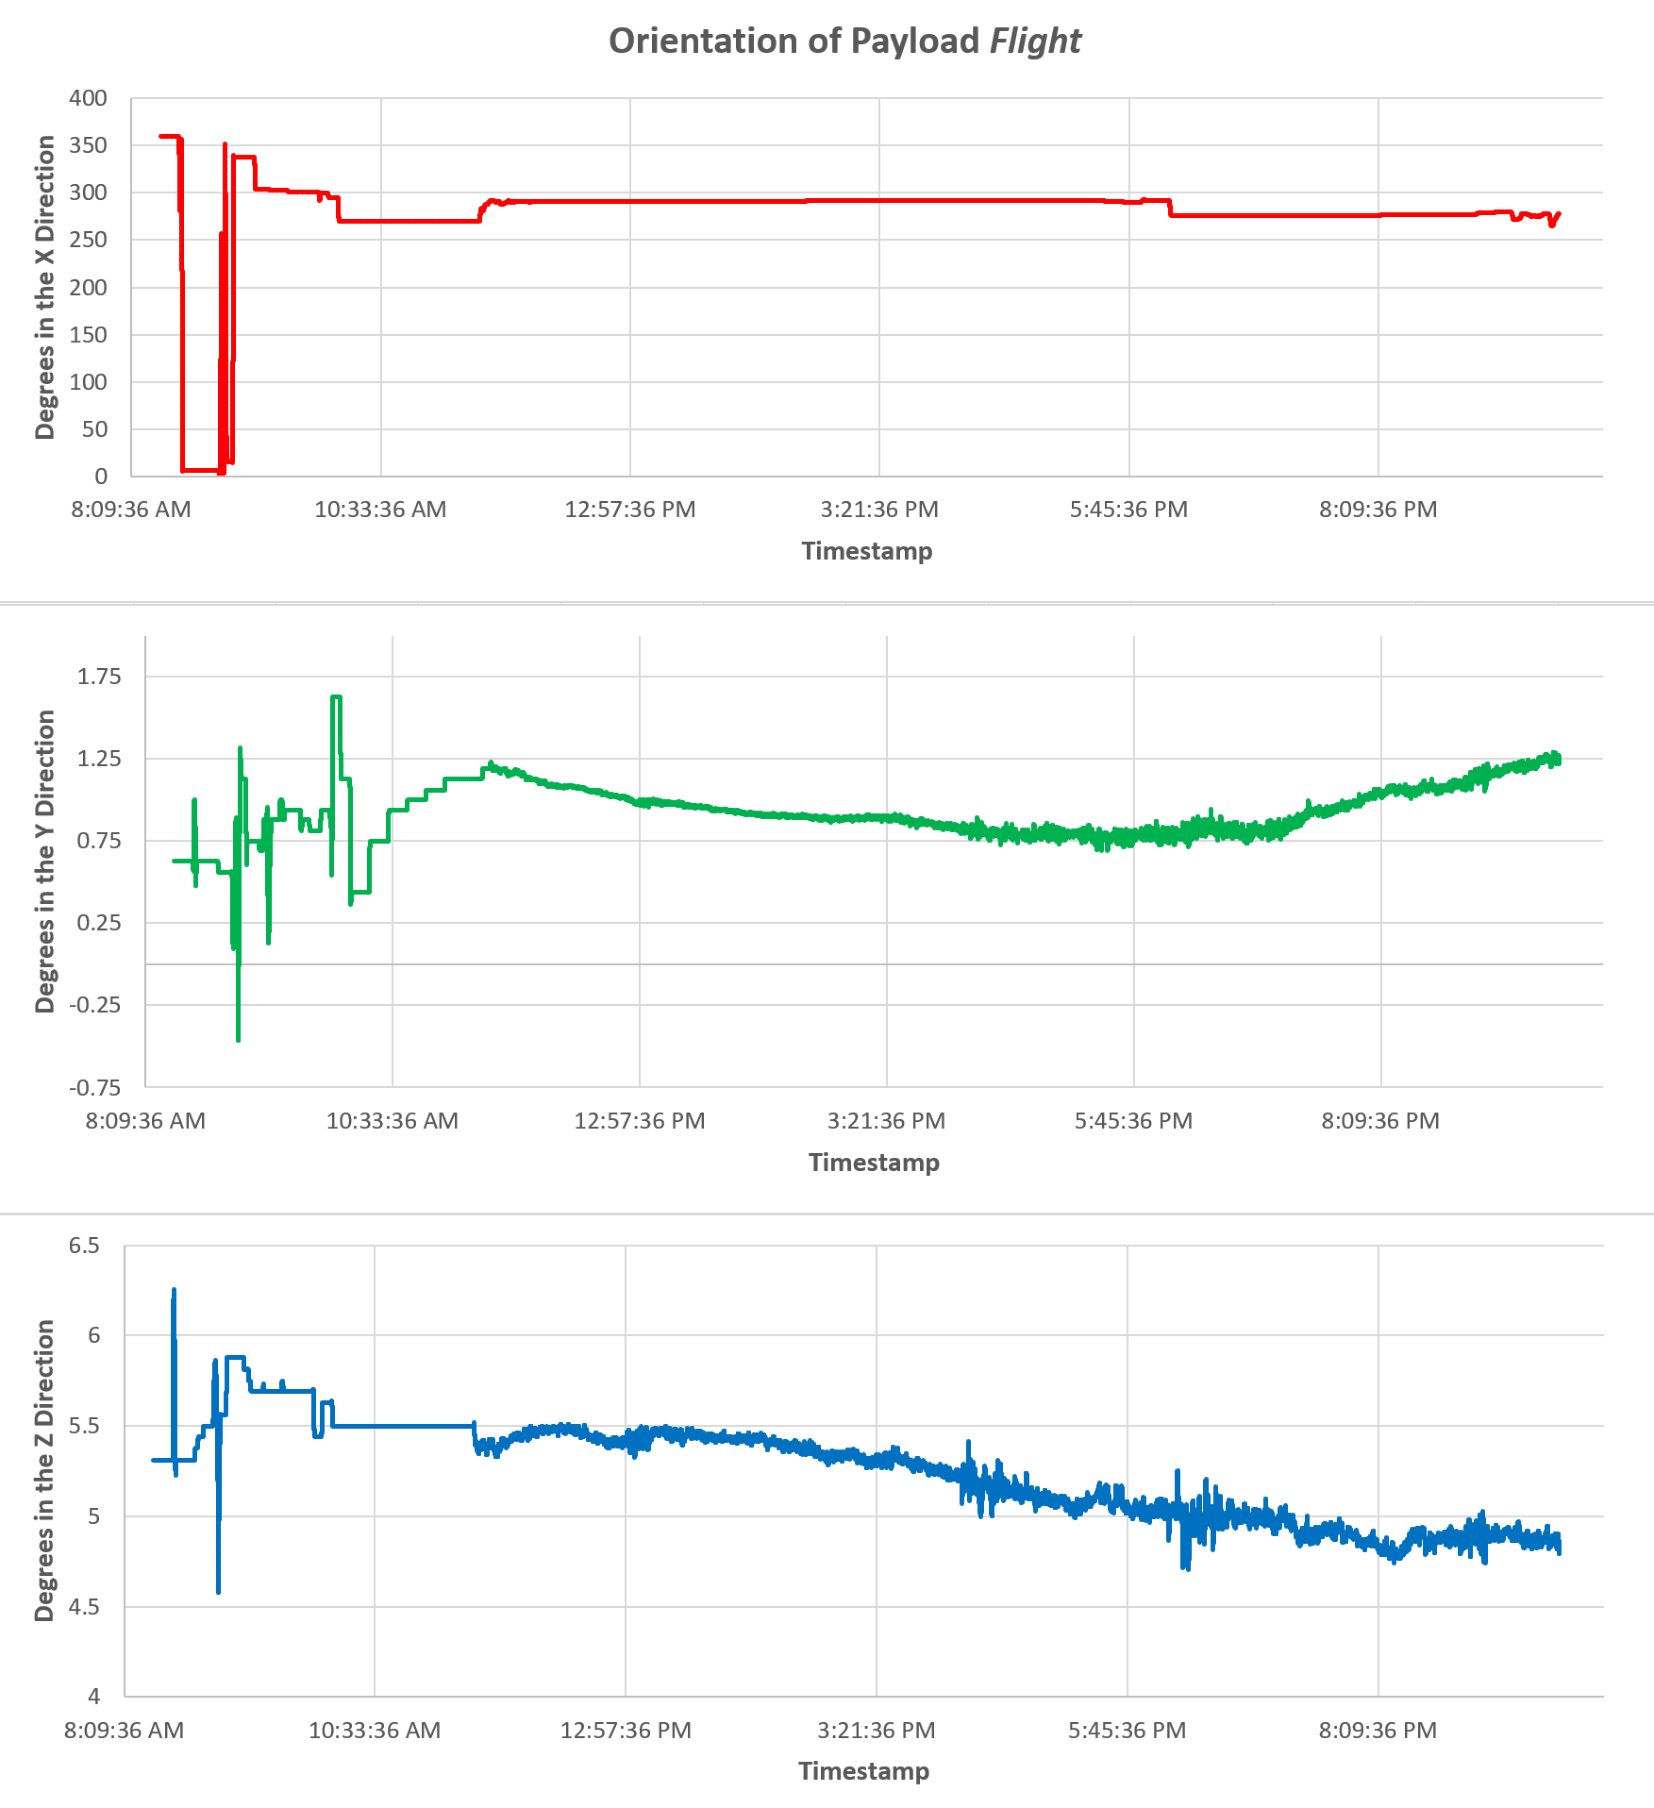
\includegraphics[width=\textwidth]{./Figures/orientation-xyz.png}
\caption{Orientation of the SORA payload in the $x, y, z$ directions.}
\label{fig:Orientation} 
\end{figure}
\clearpage
%-- 

Figure~\ref{fig:Heading} depicts the heading of the payload from true North in degrees using the BNO 6055 over Mountain Standard timestamps.  Data from the embedded magnetometer was used to create a summary of the course the payload was heading during flight.  A total of \num{359969} data entries were recorded.

\begin{figure}[H]
\centering
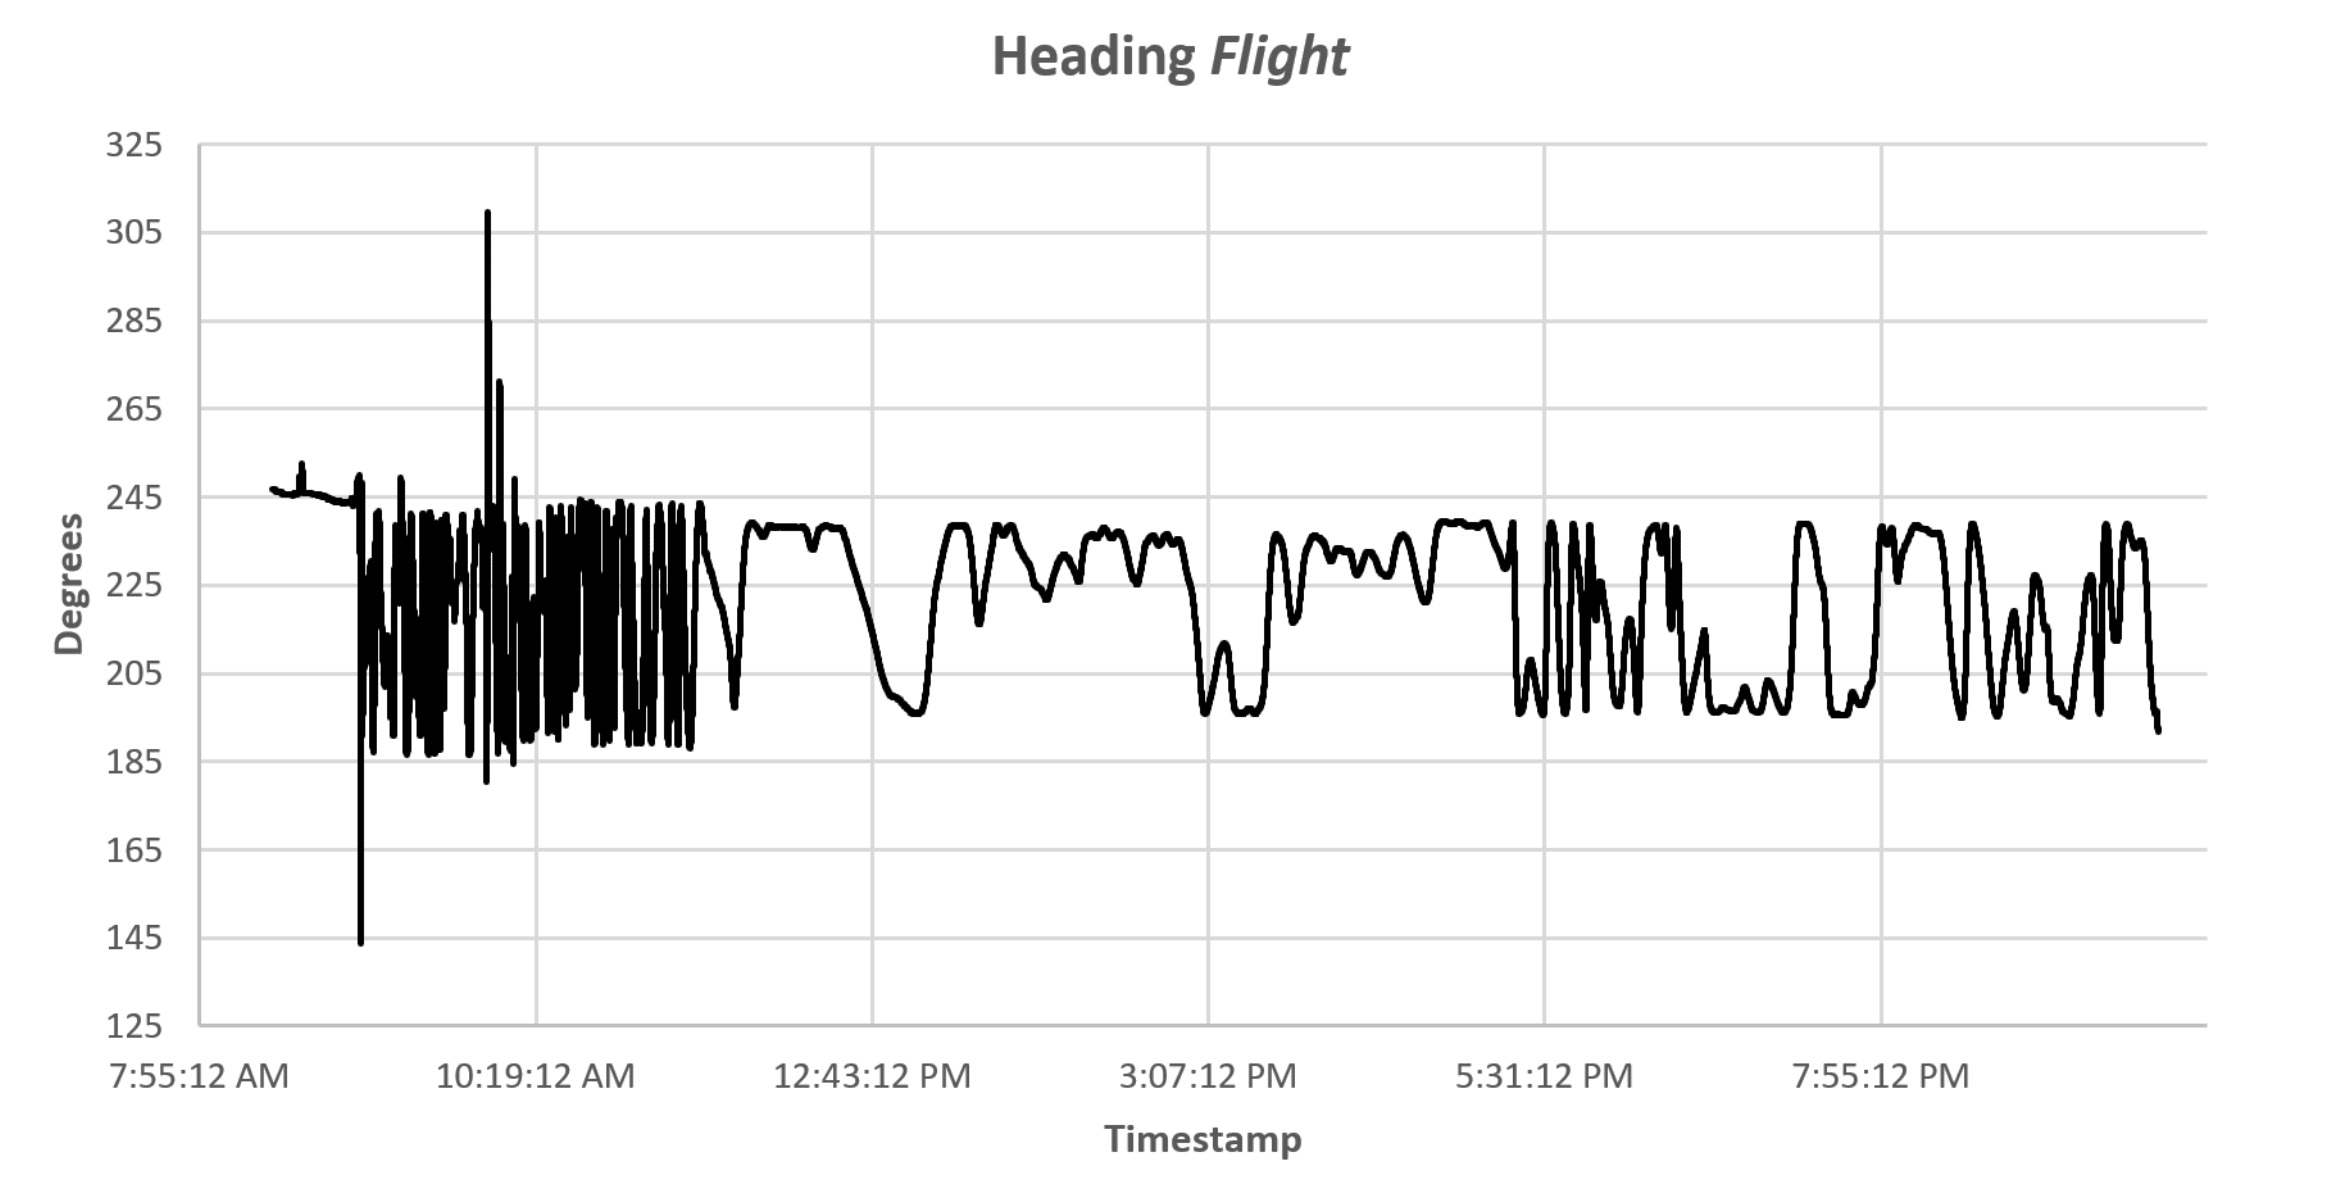
\includegraphics[width=\textwidth]{./Figures/heading.png}
\caption{Heading of the SORA payload during flight.}
\label{fig:Heading} 
\end{figure}
%-- 

%Figure~\ref{fig:Satelite-Count} depicts the number of satellites encountered during flight using the on board GPS unit 
%over Mountain standard timestamps. A total of 15,203 data entries were recorded during flight. 

%\begin{figure}[H]
%\centering
%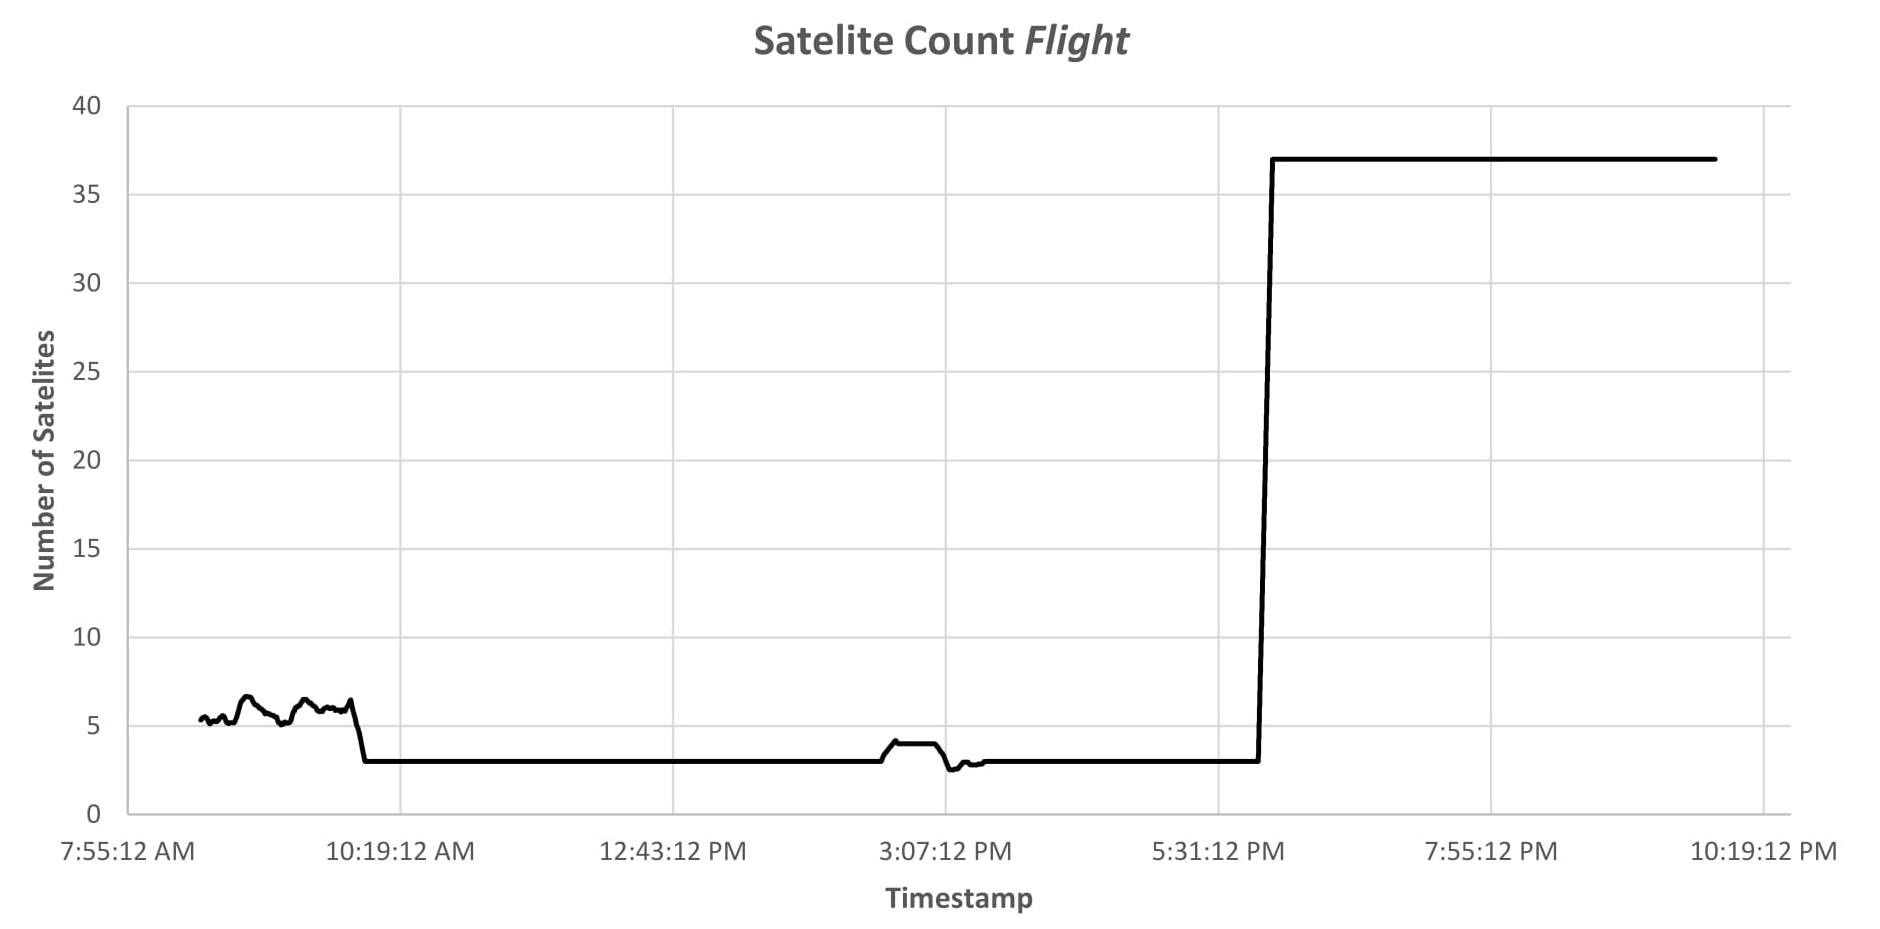
\includegraphics[scale=.25, width=\textwidth]{./Figures/SAT_COUNT.jpg}
%\caption{Number of satellites encountered by RESU over the course of the flight.}
%\label{fig:Satelite-Count}
%\end{figure}
%\clearpage 
%-- 


